\chapter{Building the Survey of the Migovec Cave System}
\begin{marginfigure}
\checkoddpage \ifoddpage \forcerectofloat \else \forceversofloat \fi
\centering
 \frame{\includegraphics[width=\linewidth]{"images/survey/compasses-jarv".jpg}} 
 \caption{Suunto instruments and their protective caves are inspected prior to leaving on expedition \pic{Jarvist Frost}}
 \label{compass}
\end{marginfigure}

\begin{quote}
`By 1996, the importance of an accurate and complete survey was apparent to all - being instrumental  in finding the connection and making a cave system' --- James `Tetley' Hooper, The Hollow Mountain, 2007. 
\end{quote}

The following article is an extension and update  on `The Survey Project' (The Hollow Mountain, 1999 chapter). It aims to describe the process of survey and map making we have followed from 2013 onwards. At the end of each expedition, a different party has collated drawings and curated the survey data before delivering a plan survey and extended elevation detailing the newest findings. To reflect this, we include each year's survey at the end of the relevant chapter.

\begin{marginfigure}
\checkoddpage \ifoddpage \forcerectofloat \else \forceversofloat \fi
\centering
 \frame{\includegraphics[width=\linewidth]{"images/survey/jarv-pss".jpg}} 
 \caption{A Permanent Survey Station is left at one of the Junctions in the cave, here detailing the updates at the pushing fronts \pic{Jarvist Frost}}
 \label{fig:PSS}
\end{marginfigure}


\section{Data collection and storage}
The skeleton of the survey project is the \emph{main line}, a 3D model which links several thousand nodes or \emph{stations}. 

Ordinarily, a station is chosen as the origin, and the spherical coordinates of each neighbouring station or node are measured in the cave: they consist of distance, inclination angle and azimuth. 

Practically, they are measured with the aid of tape measure or laster range-finder, inclinometer and compass respectively. Additionally, \emph{splay} legs are often measured: they indicate the distance to cave passage walls from the survey station of interest and do not come into the cave passage length tally; however they prove invaluable when fleshing out the cave passage geometry around survey nodes.

 \emph{Permanent Survey Stations} or PSS's are those stations where an easily found physical landmark (such as a cairn), together with descriptive, waterproof paper label exists inside the cave: these are used to `tie in' new parts of the mainline survey.

It is usual for a pair of cavers to conduct the survey by assigning the data logging to one, and instrument reading to the other. By calling out the measurements in a clear, well detached and unambiguous manner, we are able to minimise the number of typographical errors. The data is entered in pencil on waterproof logbooks (A6 format) and details for each line:

\begin{citemize}
\item direction of sighting (i.e.: from station 1 to station 2 or vice-versa)
\item distance (XX – YY)
\item azimuth (XXX)
\item inclination(±YY)
\item left, right, up, down \emph{splays}
\item direction of sighting (i.e.: from station 1 to station 2 or vice-versa)
\end{citemize}

Finally, blank pages are ideal for drawing small surveys of the newly discovered cave passage, writing additional notes, logging which survey stations.

Back on the surface, it is necessary to back up the collected measurements and `enter' the data digitally before it can be processed. Usually, the relevant pages of the survey books are photographed and filed in resealable plastic pouches and stored in a shockproof pelicase together with the bivi computer. 

\begin{marginfigure}
\checkoddpage \ifoddpage \forcerectofloat \else \forceversofloat \fi
\centering
 \frame{\includegraphics[width=\linewidth]{"images/survey/jarv-survey-notes".jpg}} 
 \caption{A excerpt of a exploration notebook after the measurements are pencilled in \pic{Jarvist Frost}}
 \label{notebook}
\end{marginfigure}

The next step, often the same evening (or morning) a group has come back to the surface, the notes are read and entered on a template text file. The file, which includes more information such as the names of the surveying party, the specific roles (ie: books or intruments), PSS location or the number of pages, is then processed by the Survex software (developed by Olly Betts from Cambridge University). By reading back the data, more typographical errors are avoided. In this step, we also specify where a specific string of survey legs should be tied into the master system. 

Over the years, we have divided the cave into different systems (\emph{Vrtnarija, Monatip} etc,…)  and regions (\passage{Apollo}, \passage{Stuck in Paradise} etc,…), which is reflected in the hierarchy of nested folders, all of which ultimately contain specific, survex-compatible \emph{.svx} files.


 \begin{figure*}[t!]
 \checkoddpage \ifoddpage \forcerectofloat \else \forceversofloat \fi
 \centering
 \begin{tikzpicture}
\node [table] (box){%
    \begin{minipage}{\textwidth}
    \begin{multicols}{2}
    \centering
\begin{verbatim}
;Apple Crumble
;Window off Povezava pitch

;Date: 24/07/17
;Instruments: James Wilson
;Book: Tanguy Racine

;Data entered by Tanguy Racine 25/07/17

;data normal bcra grade 5
;from	to	tape	comp	clino

;data on 3 pages
*begin apple_crumble
;PAGE 1/3
2	1	4.04	165	-24
3	2	5.90	134	-22
4	2	2.83	207	-09
…

;NOTES
;STN 1 IS PSS at junction of muddy crawls
;STN8 is cairn in TTT branch
;STN 9 IS PSS
;STN 7 is PSS
…

*end apple_crumble
*equate apple_crumble.26 pov.11
\end{verbatim}
\end{multicols}
  \end{minipage}
  };
\node[tabletitle, right=10pt] at (box.north west) {A typical survex file};
\end{tikzpicture}
\end{figure*}


\tdplotsetmaincoords{60}{150}
%
\pgfmathsetmacro{\rvec}{.9}
\pgfmathsetmacro{\myrvec}{0.3}
\pgfmathsetmacro{\thetavec}{-30}
\pgfmathsetmacro{\phivec}{-60}
%




\section{Processing and displays}
When the data is processed on the terminal, each \emph{station} is prefixed by the name of the enclosing file or folder. 

 \begin{verbatim} cavern pathto/asurvexfile.svx \end{verbatim} 

Therefore station 4 of \passage{Stranglehold} becomes stranglehold.4. This enables the station to be called and equated to another node to tie the survey together. 

\begin{marginfigure}
\begin{tikzpicture}[scale=4,tdplot_main_coords]
    \coordinate (O)  at (0,0,0);
    \draw[thick,->] (0,0,0) -- (-1,0,0) node[anchor=south west]{$N_{mag}$};
    \draw[thick,->] (0,0,0) -- (0,1,0) node[anchor=north west]{$E$};
\draw[thick,->] (0,0,0) -- (0,0,1) node[anchor=south]{$z$};
    \tdplotsetcoord{P}{\rvec}{\thetavec}{\phivec}
    \tdplotsetcoord{Pmid}{\myrvec}{\thetavec}{\phivec}
    \draw[-stealth] (O) node[left] {$S_k$} -- (P) node[above right] {$S_n$};
    \draw[draw = none] (O) -- (Pmid) node[above left] {r};
    \draw[dashed, color=red] (O) -- (Pxy);
    \draw[dashed, color=red] (P) -- (Pxy);
    \tdplotdrawarc{(O)}{0.2}{180+\phivec}{180}{anchor=west}{$\phi$}
    \tdplotsetthetaplanecoords{\phivec}
    \tdplotdrawarc[tdplot_rotated_coords]{(0,0,0)}{0.35}{-90}{\thetavec}%
        {anchor=south west}{$\theta$}


\end{tikzpicture}
\caption{Spherical coordinates measured inside the cave. $r$ is the distance between nodes in metres, $\theta$ is the inclination angle (\textdegree), $\phi$ is the azimuth in degrees, measured clockwise from north. Note the left-hand rule for this coordinate system.}
\end{marginfigure}

Survex begins building the mainline at a fixed origin  $(0;0;0)$.

Simple trigonometry allows that for two connected stations $S_n$ and $S_k$:
$$x_{n} = x_{k}+ r \cos\phi\cos\theta $$
$$y_{n} = y_{k}+ r \sin\phi\cos\theta $$
$$z_{n} = z_{k}+ r \sin\theta$$

 All other station coordinates in the survey file are calculated in series, relative to the origin. In case there is an indicated loop, survex distributes the error evenly across all the measured legs in the loop and this is recorded in an error log. Each individual file is processed separately before it is appended to a master, regional file such as \emph{Primadona.svx}. There, a PSS from a previous survey can be equated to a station in the new file, and a new process begins:
\begin{itemize}
\item Calculating and redistributing the errors on trans-file loops when a major connection is made
\item Correcting for each year's magnetic declination variations, (several degrees for just a decade difference)
\item checking splays and flagging up re-surveyed legs 
\end{itemize}

The output of the processing is an \emph{.3d} file displayed in \emph{Aven} software. The end product is essentially a line mesh coloured by either depth, date of exploration or loop closure error; this can be rotated 360° in the horizontal plane, 180° from top-down to bottom-up in a vertical plane. Given a surface elevation model, one can also manually check the distance from a node to the surface, or from node to node. One advantage of processing the survey datasets very early on is that the sorts of queries such as `how close are these two passages' determine the orientation of exploration during the expedition; answering them right away enables connection efforts and fuel most of the heated evening discussions about where to explore next.

In fact, the 3D viewer aven often quotes a vertical and horizontal separation between any two stations of the plot.

\begin{marginfigure}
\checkoddpage \ifoddpage \forcerectofloat \else \forceversofloat \fi
\centering
 \frame{\includegraphics[width=\linewidth]{"images/survey/surveying_colony".jpg}} 
 \caption{Will Scott surveying the climb into \protect\passage{Colony}, using compass and clinometer \pic{Tanguy Racine}}
 \label{surveying colony}
\end{marginfigure}

The main deliverable from \emph{Aven} is undoubtedly the main line; the plan view projection thereof can exported into a vector graphics software like \emph{Inkscape}. The elevation view is more intuitive because Sistem Migovec is predominantly a vertical cave system; however, a simple projection is of limited use when it comes to drawing cave passage walls around the main line. The overlapping vertical shaft series blur into one, and labelling each passage becomes an issue. Finally the horizontal distance of passages parallel with line of sight is greatly underestimated.

To overcome this problem, we produce an \emph{extended elevation}, where starting from a reference point (the cave entrance of \passage{Vrtnarija} in our case), the survey legs are unfolded into one vertical plane. The distance from station to station, and inclination angle between remain unchanged, only the azimuth is changed to either N, or S (left or right on the plane). 


\begin{figure*}[t!]
 \checkoddpage \ifoddpage \forcerectofloat \else \forceversofloat \fi
\centering
\frame{\includegraphics[width=\textwidth]{"images/maps/mig".png}}
\caption{A projection of the Migovec Cave System and LiDAR terrain data viewed in \emph{Aven}}
\label{projection}
\end{figure*}


\begin{marginfigure}
 \checkoddpage \ifoddpage \forcerectofloat \else \forceversofloat \fi
 \centering
 \begin{tikzpicture}
\node [table] (box){%
    \begin{minipage}{\textwidth}
\begin{verbatim}
;Organising Fenestrator branch
*eright prim.fenestrator.9 
*eleft prim.battery_flattery.1
*eright prim.battery_flattery.10
*eleft prim.alabaster.5
*eleft prim.sweet_baby_jesus.24
*eright prim.sweet_baby_jesus.22
\end{verbatim}
  \end{minipage}
  };
\node[tabletitle, right=10pt] at (box.north west) {Instructions};
\end{tikzpicture}
\end{marginfigure}

The major consequence of this operation is that the distance between non-adjacent nodes is no longer reflected on the visualisation software. As a corollary, long or complex loops are sometimes broken and completely unfolded. To meet the needs of the user, whether it is greater topological accuracy or the aesthetically pleasing distribution of passages on a page, it is possible to write instructions for the extension process and force a series of passage in a certain direction.

 

This is done via the following terminal command:
\begin{verbatim}
/Applications/survex/extend --specfile=instructions.dat 
   pathto/Avenfile.3d  pathto/extendedAvenfile.3d
\end{verbatim}

\begin{marginsurvey}
\frame{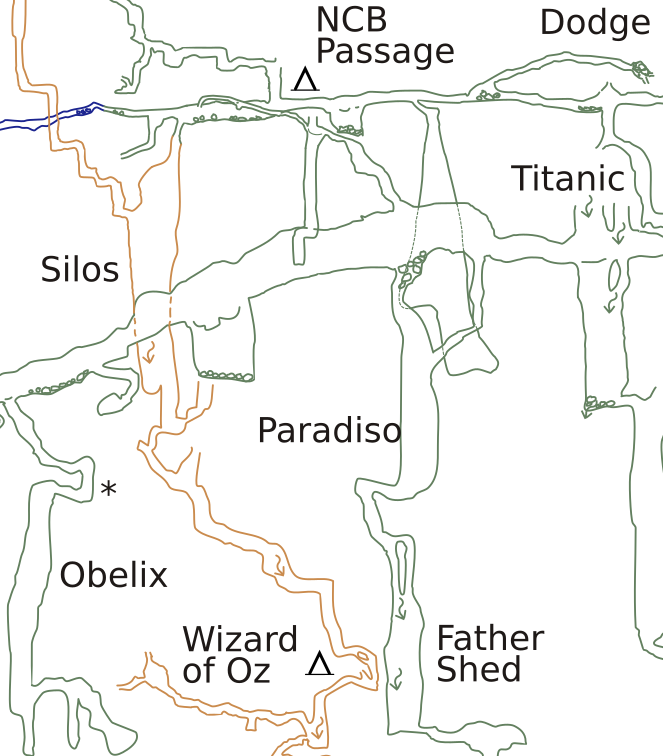
\includegraphics[width = \linewidth]{images/maps/EE_excerpt.png}}
\caption{An example of Extended Elevation survey production} \label{fig:example}
\end{marginsurvey}

creating a new, \emph{Aven} compatible .3d file, which can in turn be exported to a vector graphics software.

The instructions text file gets longer, and more complicated every year: it is the result of trial and error and a mixture of personal taste for where a passage should be and practical drawing considerations. 




\section{Making the final maps}
With a Vector Graphics Software package, it is possible to import the main line survey.The cave outline, passage walls, presence of water cascades can then be drawn around the skeleton to convey an idea of scale for the various caverns and pitches inside the cave.



By working with a cascade of well-organised layers, it is possible to hide or lock off several regions of the cave; each new addition comes under a different year label or region file. This drawing of the cave occurs after the end of an expedition, when all the grade 1 surveys drawn inside the cave or inside the bivi logbook are brought together at a survey meeting in the UK.

All newly added passage is duly annotated and labelled on plan and elevation and finally a scaled map and elevation of the cave system is submitted to the Slovene government in order to update its \emph{kataster} database. A copy can be found on the Imperial College website. \begin{verbatim} https://union.ic.ac.uk/rcc/caving/slovenia/  \end{verbatim}

\section{Geographical Information Systems}
\marginnote{Geographical Information Systems (GIS) enable the storage, display and edition of geographic information.} 

Cave entrances, with coordinates, elevation and name are instances of point data with attributes. The centrelines or main line surveys are instances of polyline data, which can be queried in several ways: the \emph{Aven} software for example enables a cursory investigation of spatial relationships between different caves, or between the cave and some surface.

Other softwares like the opensource \emph{QGIS} allow many types of georeferenced datasets to be compared and manipulated, for instance the Slovenian kataster hosts LiDAR (\emph{Light detection and Ranging}) elevation data as xyz files, and many more maps ranging from hours of sunshine per year, solid geology to official administrative boundaries and sensitive water protection areas. 

With the pursuit of speleology in mind, using the elevation data in conjunction with geological mapping can yield insights into cave system development and more rarely, potential. 

A common example of elevation data processing to produce visually appealing maps is \emph{hillshading}, or artificial illumination, which, as seen on the topographical maps within in this volume \fref{map:map overlay}, \fref{map:map area K},\fref{map:map area n} provide a qualitative appreciation of terrain. This is used in conjunction with elevation contours, which provide a quantitative measure of elevation at discrete horizons. 

In practice, in 8-bit images, a digital number between $0-255$ is assigned to each output pixel, proportional to the cosine of the 2-dimensional angle between the surface normal vector and solar illumination vector \citep{corripio2003vectorial}. 


\begin{pagemap}
\centering
\begin{subfigure}{0.76\linewidth}
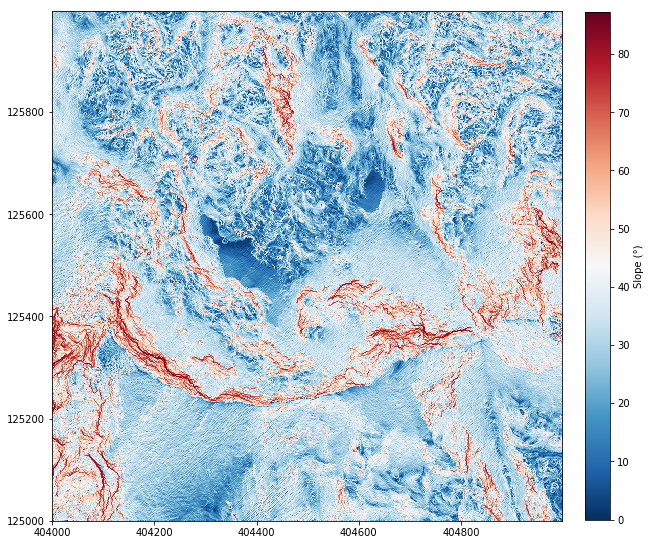
\includegraphics[width = \textwidth]{images/maps/slopemap.png}
\subcaption{ } \label{slope}
\end{subfigure}

\begin{subfigure}{0.76\linewidth}
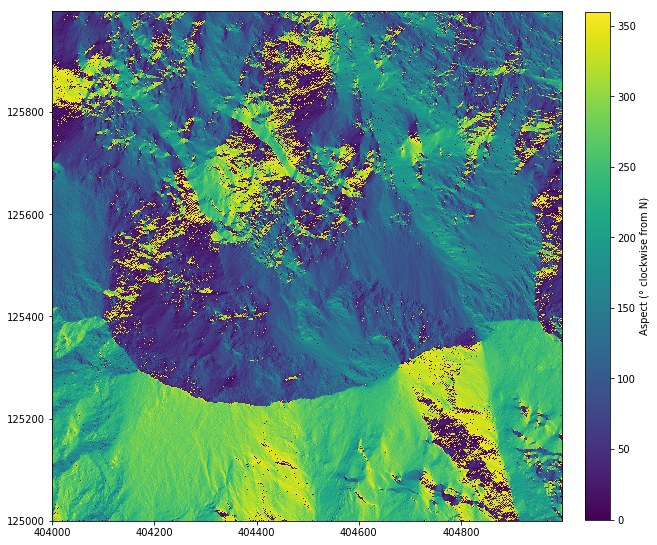
\includegraphics[width = \textwidth]{images/maps/aspectmap.png}
\subcaption{ } \label{aspect}
\end{subfigure}

\caption[Slope and Aspect maps]{Examples of  \emph{(top)} slope and  \emph{(bottom)} aspect maps generated from simple elevation data. The area is 1km x 1km over \protect\passage{Tolminski Kuk} --- Slovenia National Grid EPSG 3794}
\end{pagemap}







